\chapter{Interception HTTPS}

\label{sec:https-interception}

\begin{figure}[H]
  \caption{Attaque HTTPS interception (diagramme Dia)}
  \fbox{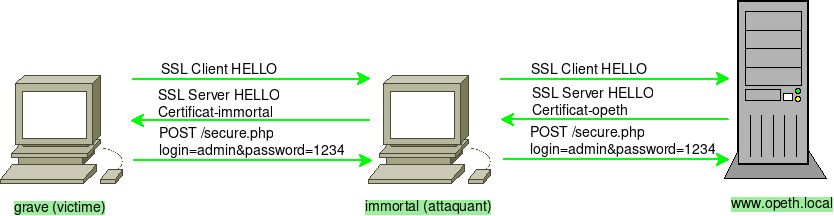
\includegraphics[width=\textwidth]{../medias/https-interception/attack.png}}
\end{figure}

\section{Description de l'attaque}

La méthode que nous allons voir pour intercepter un trafic HTTPS n'est pas vraiment une attaque. Pour être menée à bien, la machine, placée en homme du milieu, doit avoir installée sa propre autorité de certification, et surtout l'avoir rentrée sur la machine du client, en amont.

C'est une chose qui peut être assez dure à réaliser pour un attaquant, mais il existe des cas où cette situation se trouve. Dans le cadre d'une entreprise, il n'est pas rare que les requêtes HTTP des employés passent par un proxy, pour suivre leurs activités. Les responsables n'ont par contre, a priori pas moyen de lire les requêtes HTTPS, du moins c'est ce qu'on pourrait penser.

Car c'est en fait au contraire assez simple à réaliser dans la mesure où il est facile de rajouter une autorité de certification à la main dans les navigateurs web de tous les employés.

L'idée de la méthode est d'agir comme un simple proxy HTTPS. Lors de la connexion initiale du client vers le site web, la machine placée en homme du milieu va récupérer la requête, et établir elle même une connexion avec le serveur distant. Le proxy n'a plus qu'à établir une connexion avec le client, ce qui ne pose pas de problème car l'autorité de certification est acceptée par le navigateur du client.

L'ANSSI a d'ailleurs publié une ressource à destination des entreprises sur comment intercepter le traffic https de ses employés : \url{https://www.ssi.gouv.fr/uploads/IMG/pdf/NP_TLS_NoteTech.pdf}
\section{Notre attaque}

\subsection{Mise en place de l'environnement}

Le serveur \textbf{opeth} héberge deux pages sur le domaine \path{www.opeth.local} :

\begin{itemize}
\item une page \path{index.php} que l'on accède en HTTPS et présentant un formulaire de login ;
\item une page \path{secure.php} que l'on accède en HTTPS depuis la page \path{index.php}.
\end{itemize}

Pour la résolution DNS, nous utilisons simplement le fichier \path{/etc/hosts} de chaque machine. Nous avons également mis en place HSTS sur cette attaque, étant donné que nous traitons uniquement des flux HTTPS.

\subsection{Démonstration}

Pour lancer l'environnement de test, il faut lancer la commande suivante (on aura récupéré au préalable le dépôt qemunet) :

\begin{minted}{bash}
./qemunet/qemunet.sh -x -S https-interception
\end{minted}

À partir de là, les trois machines sont lancées.

\subsubsection{Étape 1 : avant l'attaque}

Avant que l'attaque soit lancée, nous pouvons accéder à la page de login de manière sécurisée. La machine immortal n'est pas capable de comprendre la communication entre le client (grave) et le serveur (opeth) :

\begin{figure}[H]
  \caption{Attaque https-interception (avant l'attaque)}
  \fbox{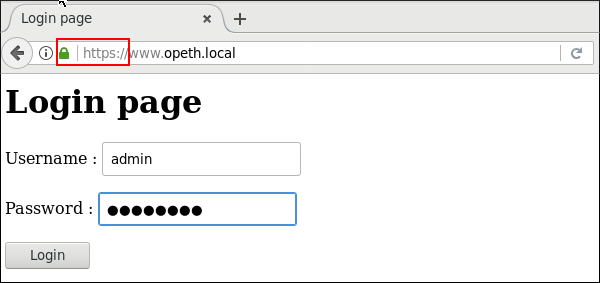
\includegraphics[width=\textwidth]{../medias/https-interception/screen1.png}}
\end{figure}

Ici, on voit que c'est bien le certificat du serveur qui est présenté au navigateur :

\begin{figure}[H]
  \caption{Certificat}
  \fbox{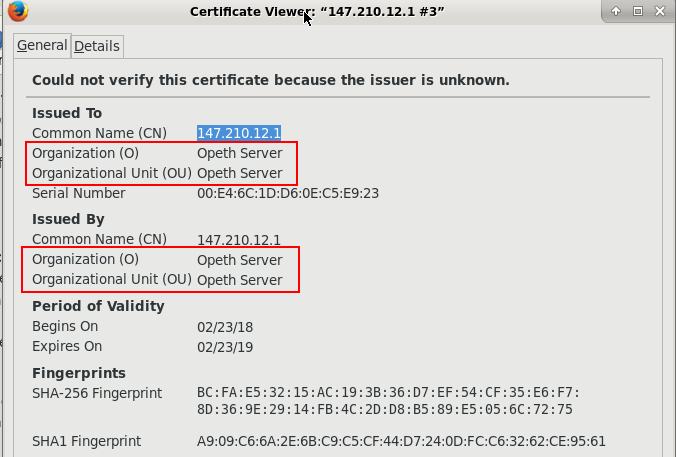
\includegraphics[width=\textwidth]{../medias/https-interception/screen2.png}}
\end{figure}

Nous voici sur la page secure.php, nos données ont transitées de manière chiffrées entre le client et le serveur :

\begin{figure}[H]
  \caption{HTTPS se présente normalement}
  \fbox{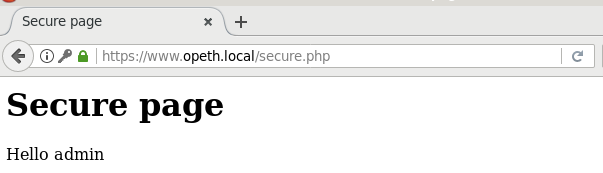
\includegraphics[width=\textwidth]{../medias/https-interception/screen3.png}}
\end{figure}


\subsubsection{Étape 2 : lancement de l'attaque}

Comme expliqué précédemment, pour lancer l'attaque, il faut exécuter le fichier \path{/mnt/host/attack.sh} depuis immortal. Voici son contenu :

\begin{minted}{bash}
PROXY_PORT=4242

iptables -t nat -F
iptables -t nat -A PREROUTING -d 147.210.12.1 -p tcp --dport 443 -j REDIRECT --to-port $PROXY_PORT
/mnt/host/https-interception.py $PROXY_PORT
\end{minted}

On peut constater que les flux TCP à destination du port 443 (HTTPS) sont redirigées vers le port d'écoute du proxy qui est chargé d'analyser et traiter les requêtes.

Sur la machine immortal, nous lançons le script de l'attaque :

\begin{figure}[H]
  \caption{Lancement de l'attaque}
  \fbox{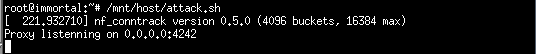
\includegraphics[width=\textwidth]{../medias/https-interception/screen4.png}}
\end{figure}

\paragraph{Explication du code du proxy \\}

Le code du proxy est dans le fichier \path{https-interception.py}. Ce dernier est sensiblement le même que celui utilisé pour l'attaque SSLStrip.

\subparagraph{Contexte SSL du proxy \\}

Le proxy doit ajouter son certificat au contexte pour pouvoir le présenter au client :

\begin{minted}{python}
def __listen(self):
	sock = socket.socket()
	context = ssl.create_default_context(ssl.Purpose.CLIENT_AUTH)
	context.load_cert_chain(certfile=PROXY_CERT, keyfile=PROXY_KEY)
	...
\end{minted}

\subsubsection{Étape 3 : pendant l'attaque}

Lorsque l'attaque est en cours, le certificat présenté au client n'est plus celui d'opeth, mais celui du Proxy, signé par l'autorité de certification. À noter qu'ici si l'autorité de certification du proxy n'avait pas été présent dans le navigateur, celui-ci aurait émis une alerte.

Ci-dessous on voit que le certificat présenté est celui du proxy (immortal), et non plus celui du serveur. On voit bien que les empreintes SHA256 sont différentes.

\begin{figure}[H]
  \caption{Le certificat a changé}
  \fbox{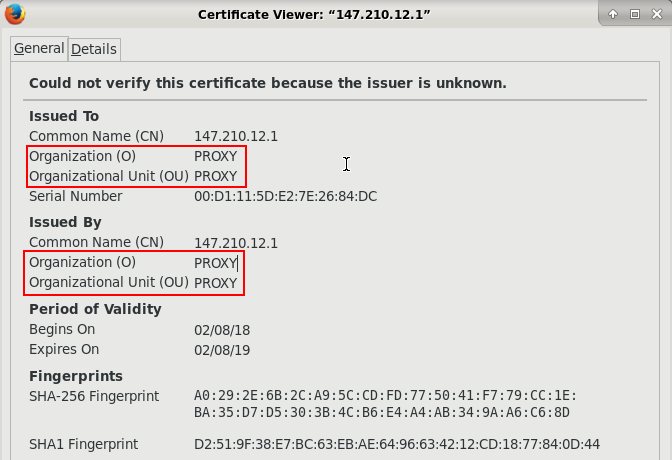
\includegraphics[width=\textwidth]{../medias/https-interception/screen6.png}}
\end{figure}

Si le certificat est accepté par le client et que nous essayons de nous enregistrer :

\begin{figure}[H]
  \caption{Connexion sécurisée}
  \fbox{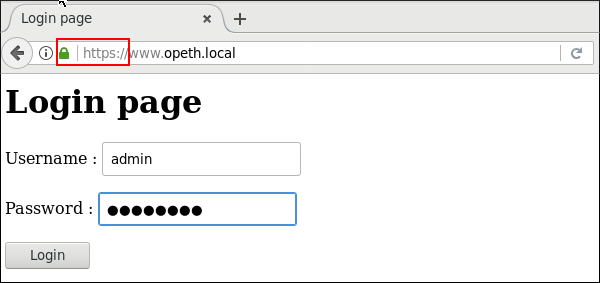
\includegraphics[width=\textwidth]{../medias/https-interception/screen1.png}}
\end{figure}

Nous arrivons bien sur la page secure.php, et notre connexion est bien effectuée en HTTPS. Le client n'a constaté aucun changement au niveau de sa navigation.

\begin{figure}[H]
  \caption{Tout a l'air normal pour le client}
  \fbox{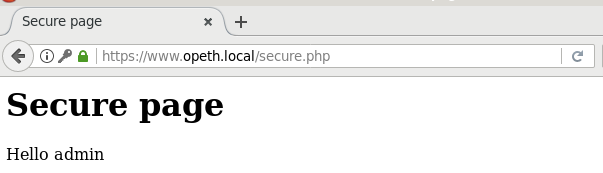
\includegraphics[width=\textwidth]{../medias/https-interception/screen3.png}}
\end{figure}

Par contre, la machine immortal a jouée le rôle d'un proxy et a été capable de récupérer la communication en clair. Ici on voit que le nom d'utilisateur, le mot de passe ainsi que le cookie de session ont pût être capturés :

\begin{figure}[H]
  \caption{L'attaquant a intercepté les informations sensibles}
  \fbox{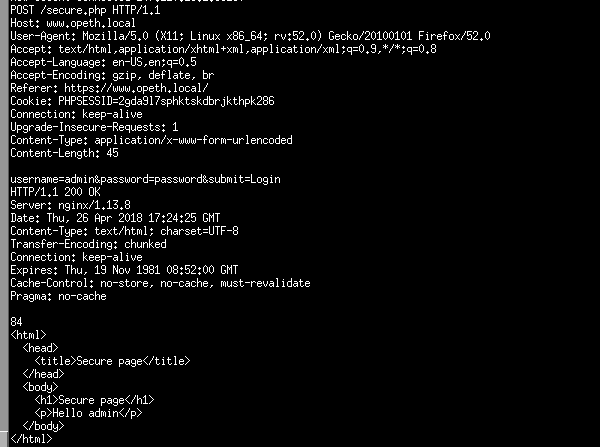
\includegraphics[width=\textwidth]{../medias/https-interception/screen9.png}}
\end{figure}

Le script complet de l'attaque peut être consulté à l'annexe \ref{appendix:https-interception}.

\section{Limitations de notre attaque}

Notre attaque étant une preuve de concept, celle-ci présente un certain nombre de limitations. Dans un premier temps, nous avons supposé qu'il était possible d'installer un certificat sur le navigateur du client. Ceci est bien entendu possible pour les administrateurs de postes clients d'une entreprise. Certains antivirus utilisent également cette technique afin d'analyser le trafic HTTPS d'une machine.

Mais dans la majorité des cas, ceci n'est pas une option. Pour contourner ce problème, soit l'attaquant proposera un certificat qui ne pourra pas être signé par une autorité de certification, et alors celui-ci déclenchera alors une alerte sur le naviguateur du client concerné. Soit l'attaquant cherchera à pirater une autorité de certification publique, dans le but de générer des certificats frauduleux pour des domaines légitimes. Cette dernière possibilité est sans doutes la plus compliquée et la moins réaliste.
